\documentclass[a4paper,12pt]{article} % Use article class, A4 size, and 12pt font

% Packages
\usepackage[utf8]{inputenc} % For UTF-8 encoding
\usepackage{amsmath, amssymb} % Math symbols
\usepackage{graphicx} % For including images
\usepackage{geometry} % For customizing page layout
\usepackage{hyperref} % For clickable links and references
\usepackage{setspace} % For line spacing
\usepackage{fancyhdr} % For custom headers and footers
\usepackage{lipsum} % For dummy text
\usepackage{listings}
\usepackage{xcolor}
\usepackage{xcolor-material}

% Page layout
\geometry{margin=1in} % 1 inch margins

% Header and footer
\pagestyle{fancy}
\fancyhf{}
\fancyhead[L]{Laporan Progress Sistem Tertanam} % Left header text
\fancyhead[R]{\thepage} % Right header with page number

\lstdefinestyle{mystyle}{
    backgroundcolor=\color{white},   
    commentstyle=\color{green},
    keywordstyle=\color{magenta},
    numberstyle=\tiny\color{gray},
    stringstyle=\color{purple},
    basicstyle=\ttfamily\footnotesize,
    breakatwhitespace=false,         
    breaklines=true,                 
    captionpos=b,                    
    keepspaces=true,    
    numbers=none,                              
    numbersep=5pt,                  
    showspaces=false,                
    showstringspaces=false,
    showtabs=false,                  
    tabsize=2,
}

\lstset{style=mystyle}

\title{Laporan Progress\\Menampilkan Text pada \textit{Dot Matrix}}
\date{}

\begin{document}
\begin{titlepage}
    \centering
    \vspace*{1cm}
    
     {\Large \textbf{Laporan Progress Menampilkan Text pada \textit{Dot Matrix Display}}}

    \vfill
    \vspace{2cm}

    
\includegraphics[width=0.4\textwidth]{./logo.png} % Replace <path_to_logo> with the path to your ITS logo image
    \vfill

    \vspace{1cm}
    \begin{onehalfspace}
    \textbf{Dosen Pengampu}\\
    Eko Pramunanto,S.T. M.T.

    \vspace{1cm}

    \textbf{Disusun Oleh:}\\
    Muhammad Haekal Muhyidin Al-Araby\\ 
    5024221004\\
    Sistem Tertanam - A
    \end{onehalfspace}

    \vfill

    \textbf{DEPARTEMEN TEKNIK KOMPUTER\\
    FAKULTAS TEKNOLOGI ELEKTRO DAN INFORMATIKA CERDAS\\
    INSTITUT TEKNOLOGI SEPULUH NOPEMBER\\2024}
\end{titlepage}

% Sections
\section{Komponen}
\begin{enumerate}
    \item ESP32\\
    ESP32 sebagai mikrokontroller yang digunakan untuk mengendalikan dotmatrix
    melalui program yang telah dipasang atau flash. 
    \item MAX7219 8x32 LED Dot Matrix Display Module\\
    Modul terdiri dari 4 buah dot matrix dan IC MAX7219 yang digunakan untuk sebagai 
    penghubung antara ESP32 dan display dotmatrix. Bertindak sebagai decoder dan selector.
    \item PCB\\
    Sebagai tempat untuk merangkai barang yang ada dan menyambungkannya.
    \item Pin Header Female\\
    Untuk menghubungkan ESP32 dengan PCB.
    \item Pin Header Male Siku\\
    Menghubungkan display ke PCB
\end{enumerate}

\section{Desain Sistem}
\subsection{Rangkaian Skematik}
\begin{figure}[h]
    \centering
    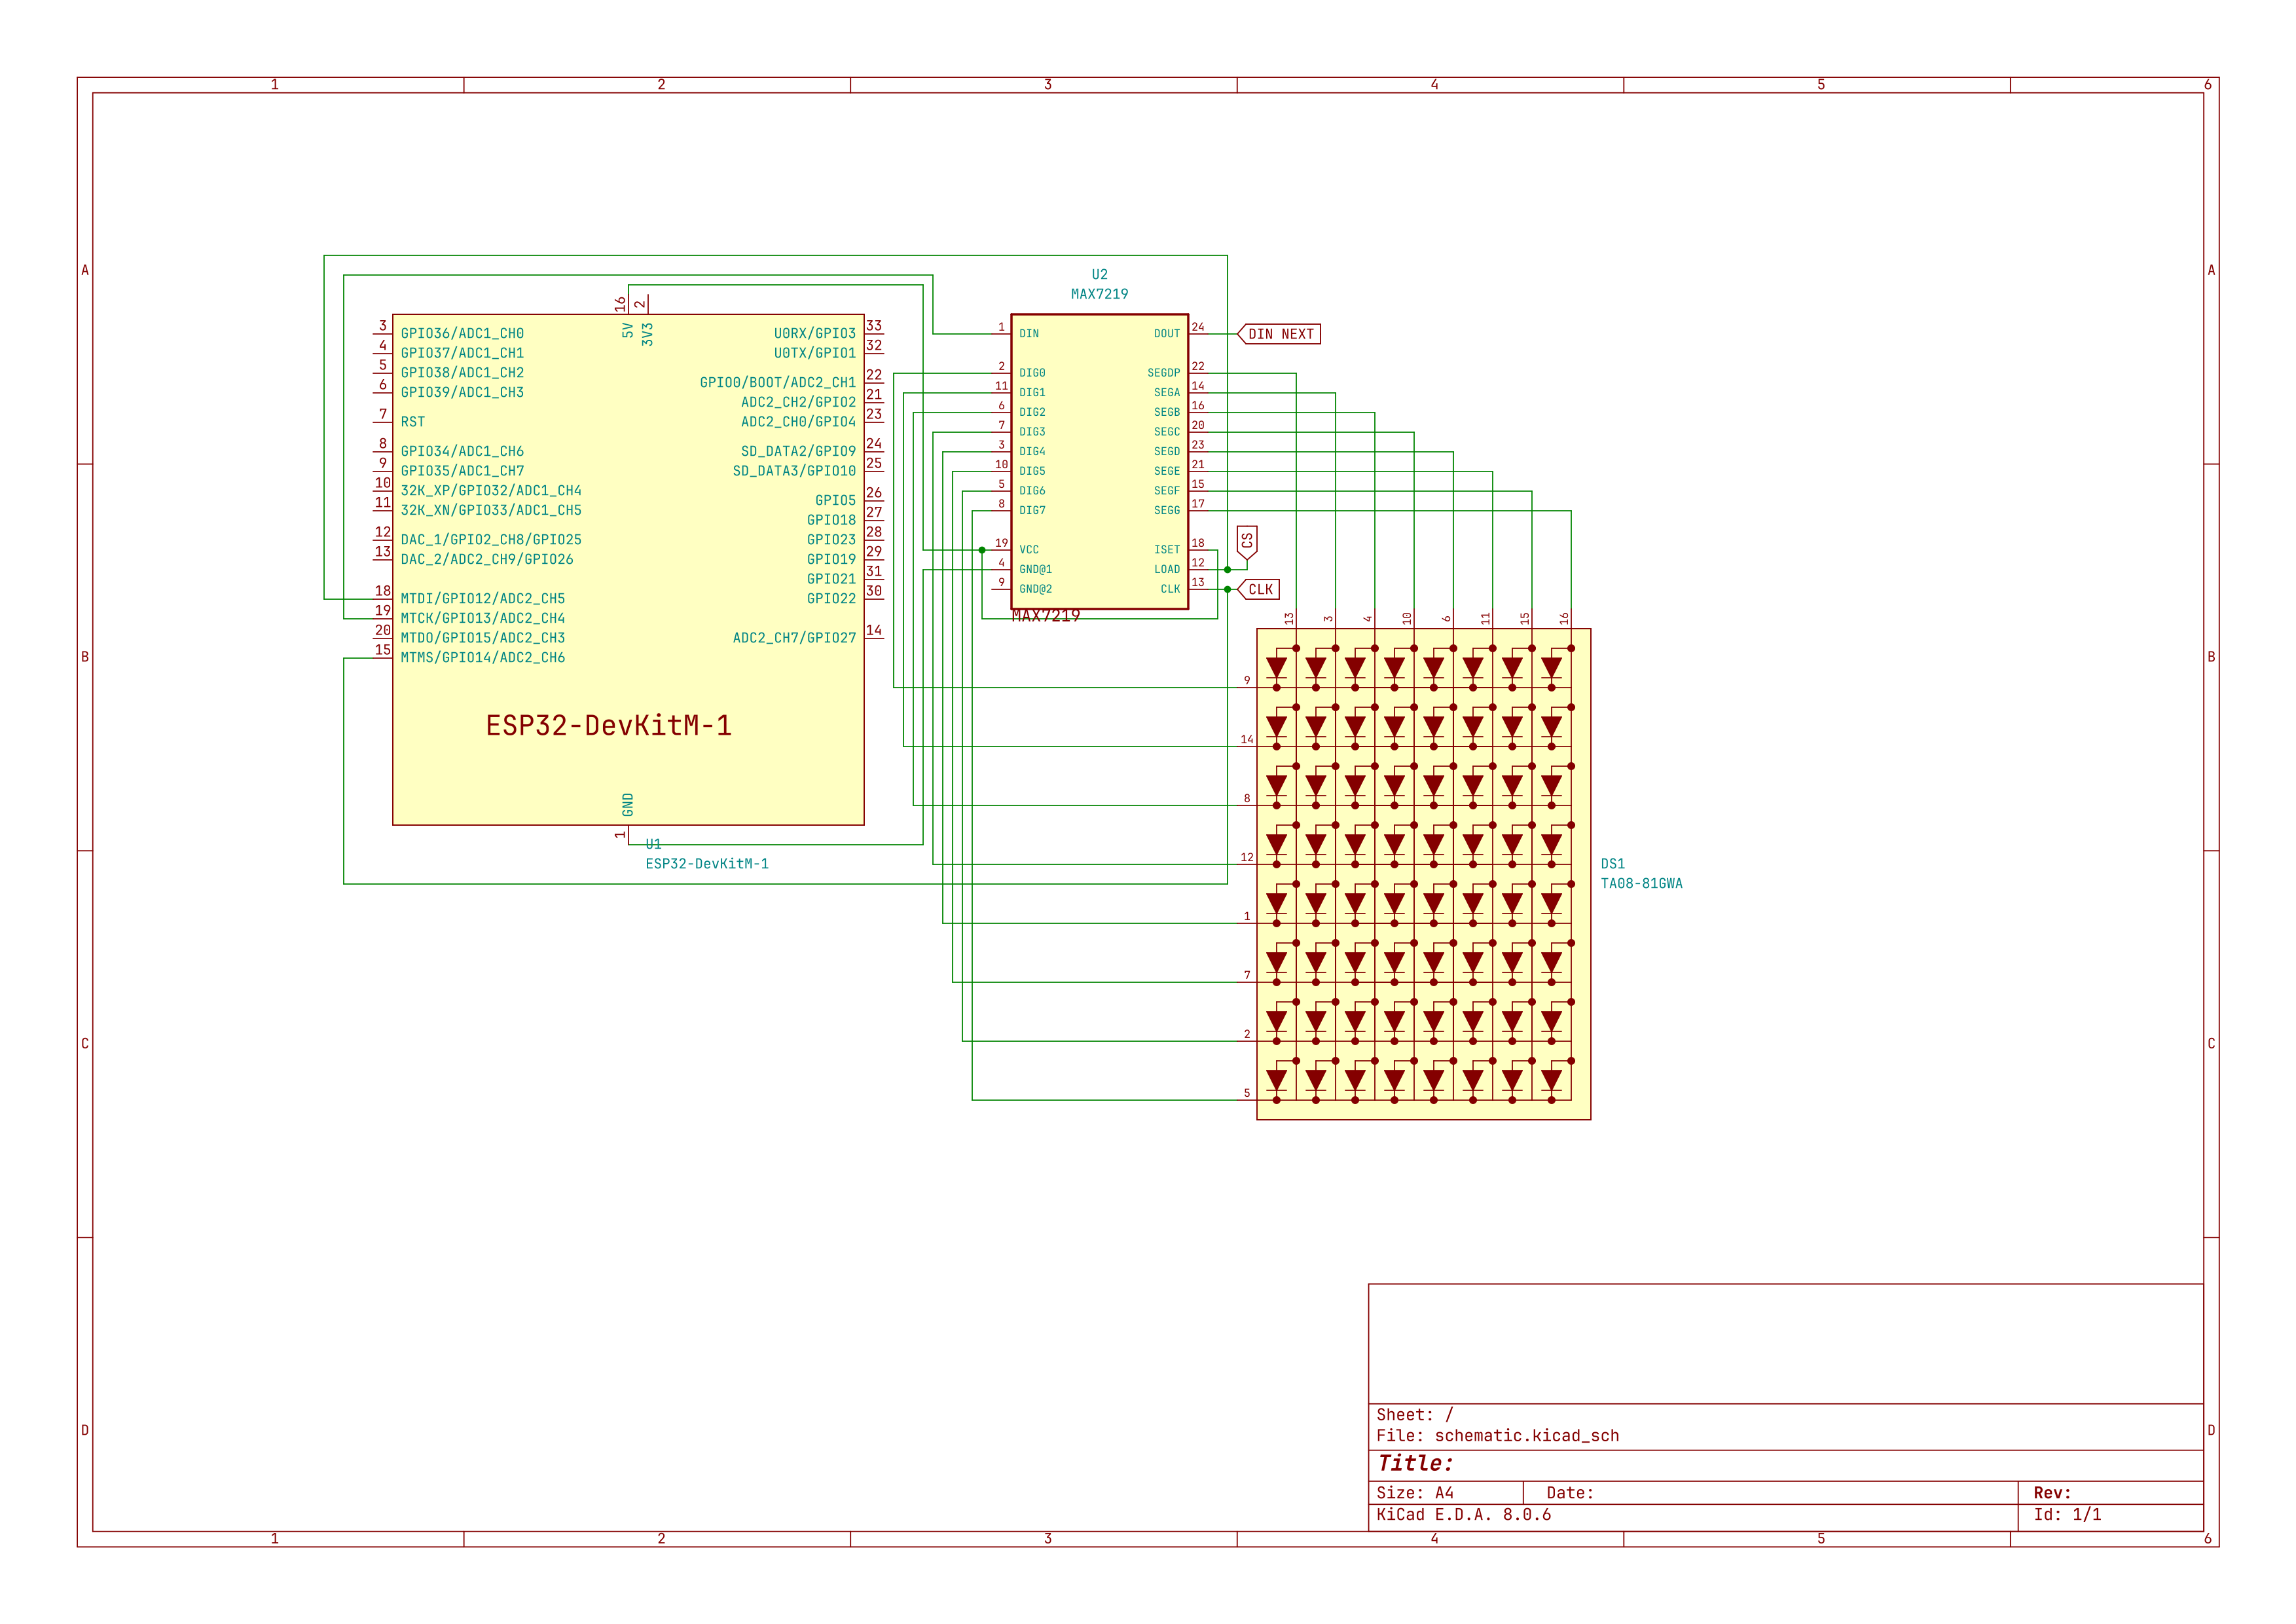
\includegraphics[width=1\textwidth]{schematic.png} 
    \label{fig:schematic}
\end{figure}
Rangkaian menggunakan ESP32 yang terhubung pada IC MAX7219 dimana CS 
terhubung pada pin D12, DIN pada D13 dan clock pada D14
terdapat 4 IC MAX7219 yang saling terhubung secara seri.

\subsection{Kode Program}
\lstinputlisting[language=C++]{main.cpp}
\section{Mekanisme Alat}
Define pin yang ESP32 yang terhubung pada IC MAX7219. Lalu define Hardware yang digunakan
buat instance object dari class \texttt{MD\_Parola} untuk mengendalikan display dengan scroll text, 
dan instance dari class \texttt{MD\_MAX72XX} untuk mengendalikan display secara langsung. Pada setup panggil
fungsi \texttt{begin} pada kedua class lalu pertama menyalakan display secara berurutan per baris dan per kolom
dengan \texttt{MD\_MAX72XX} lalu setelah selesai hanya tinggal memanggil \texttt{displayScroll} untuk menampilkan string
lalu sebelum itu bisa set \texttt{intensity} untuk mengatur kecerahan dari LED.
Pada fungsi \texttt{loop} hanya perlu display reset setelah animasi selesai.

\section{Alat}
\begin{figure}[h]
    \centering
    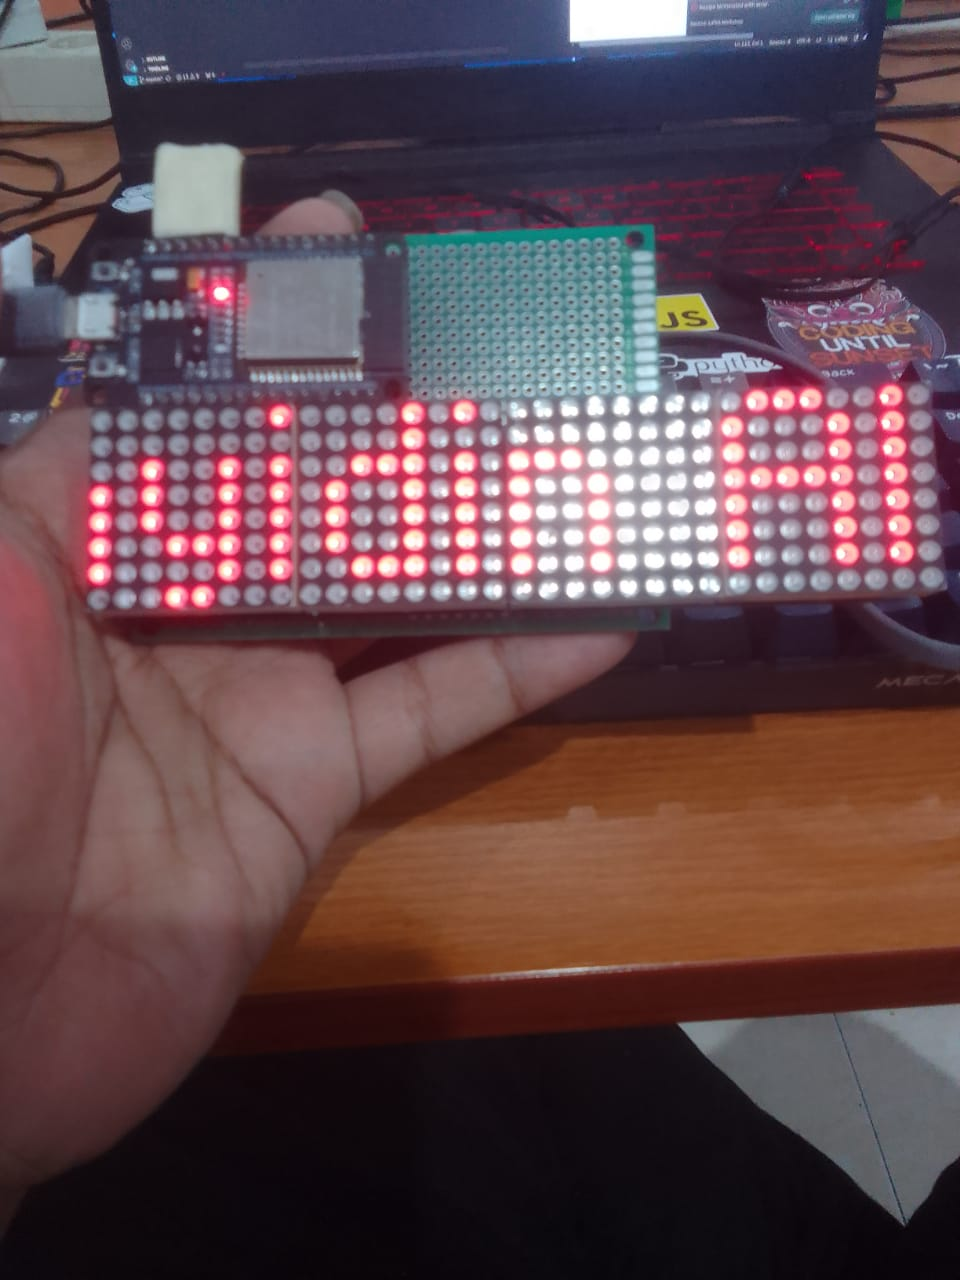
\includegraphics[width=0.5\textwidth]{alat.jpeg} 
    \label{fig:alat}
\end{figure}
\end{document}
